\documentclass[11pt,a4paper]{article}
\usepackage[T1]{fontenc}
\usepackage[utf8]{inputenc}
\usepackage{lmodern,microtype}
\usepackage[margin=27mm]{geometry}
\usepackage{amsmath,amssymb,amsthm,mathtools,bm}
\usepackage{booktabs,array,graphicx,enumitem,xcolor}
\usepackage{fancyhdr}
\usepackage[hyphens]{url}
\usepackage[colorlinks=true,linkcolor=blue!45!black,citecolor=blue!45!black,urlcolor=blue!45!black]{hyperref}
\usepackage[nameinlink,noabbrev]{cleveref}
\newtheorem{theorem}{Theorem}[section]
\newtheorem{proposition}[theorem]{Proposition}
\newtheorem{lemma}[theorem]{Lemma}
\newtheorem{corollary}[theorem]{Corollary}
\theoremstyle{remark}
\newtheorem{remark}[theorem]{Remark}
\newtheorem{example}[theorem]{Example}
\DeclareMathOperator{\Alt}{Alt}
\DeclareMathOperator{\GL}{GL}
\DeclareMathOperator{\Sp}{Sp}
\DeclareMathOperator{\rank}{rank}
\DeclareMathOperator{\supp}{supp}
\newcommand{\E}{\mathbb E}
\newcommand{\F}{\mathbb F_q}
\newcommand{\Pbb}{\mathbb P}
\setlist{itemsep=3pt,topsep=6pt}
\setlength{\emergencystretch}{2em}
\pagestyle{fancy}
\fancyhf{}
\fancyhead[L]{\small Hidden symplectic forms}
\fancyhead[R]{\small Sharp detection and recovery}
\fancyfoot[C]{\thepage}
\setlength{\headheight}{14pt}
\hypersetup{pdftitle={Recovering a Hidden Symplectic Form},pdfauthor={Research collaboration for Vladimir Reshetnikov},pdfsubject={Sharp additive detection and recovery threshold from random isotropic planes}}
\title{\textbf{Recovering a Hidden Symplectic Form}\\[5pt]
\large A sharp additive threshold for isotropic-plane observations}
\author{Research note prepared for Vladimir Reshetnikov}
\date{27 November 2026}
\begin{document}
\maketitle
\begin{abstract}
An unknown nondegenerate alternating form on $\mathbb F_q^n$ is shared by a collection of random two-dimensional subspaces, each isotropic for that form. After averaging over the hidden form, one observation is exactly uniform on all two-planes. We prove that the collective observations undergo a sharp statistical and algorithmic transition at $d=\binom n2-1$. For fixed $q$ and even $n\to\infty$, $d-\omega(1)$ observations are asymptotically indistinguishable from independent uniform two-planes, and every estimator has vanishing probability of recovering the form. At $d+\omega(1)$ observations, Gaussian elimination recovers it up to scalar with probability tending to one. We give explicit finite-dimensional bounds and the exact critical-window second moment $\chi^2\to q^a/c_q$ at $t=d+a$, where $c_q=\prod_{j\ge2}(1-q^{-(2j-1)})$. The experiment is exactly equivalent to full-row-rank wide symplectic compression with a shared unknown source form. This answers a specified case of an open question in the ProveIt GRH article. All proofs are unconditional and include characteristic two. Exact enumeration accompanies the arguments.
\end{abstract}
\tableofcontents
\newpage

\section{Origin, contribution, and interpretation}

The ProveIt project studies both consequences of Dirichlet GRH and transfers of the mechanisms appearing in its source proof. Its current article includes exact laws for symplectic matrix compressions, and asks about observations with a shared unknown source form \cite[\texttt{spn:q:symplectic}]{proveit}. The present paper develops that question into a statistical recovery problem and proves a matching lower and upper sample threshold.

The source revision used throughout is
\begin{center}\small
\nolinkurl{00cadb961bbe77c74e5d082c4948f8884d58a970}.
\end{center}
At this revision the article consolidates 184 reports, while ten further packets remain under \texttt{Research/}. We inspected the article's source and the additional symplectic packets before selecting this problem. Their results concern specified source forms, individual block distributions, rank blindness, and joint rank--defect laws. The hidden common-form experiment studied here is different: averaging hides all evidence in a single retained observation, but repeated observations constrain the same unknown form.

An alternating form is an array of pairwise interaction coefficients $H_{ij}$ with $H_{ii}=0$ and $H_{ji}=-H_{ij}$. It assigns an area-like quantity $H(u,v)$ to two vectors. The observed plane $\langle u,v\rangle$ tells us that this quantity vanishes. It supplies one linear equation in the $\binom n2$ coefficients. Rescaling all coefficients is unobservable, so $d=\binom n2-1$ is the natural parameter count. Parameter counting alone does not prove the theorem: the equations come from decomposable exterior products and are highly structured. A proof must control exceptional competing forms and must show that the hidden mixture is statistically invisible below the threshold.

The principal contributions are the additive threshold, its information-theoretic lower bound, recovery by Gaussian elimination at the same scale, and an exact limiting second moment in the bounded window. The incidence geometry and the Pl\"ucker description of symplectic Grassmannians are classical; related point counts occur in the work of Blok and of Cardinali--Giuzzi \cite{blok,cardinali}. Our proofs reproduce the counts needed here. A targeted literature search did not identify the exact shared-form threshold, but this is a research contribution relative to the inspected sources, not a claim of an exhaustive priority search.

The new results do not use RH or GRH. The connection with that research program is through the article's symplectic compression mechanism and its explicit open question. The upstream Lean development is not rebuilt in this work, and the present proof is a mathematical proof with exact computational checks, not a completed Lean formalization.

% Standalone mathematical body; standard amsmath/amsthm notation.
% Suggested macros: \F=\mathbb F_q, \Pbb=\mathbb P, \E=\mathbb E,
% \Alt=\operatorname{Alt}, \TV=d_{\rm TV}.

\section{A hidden symplectic form: the statistical experiment}

Fix a prime power $q$, an even integer $n\ge4$, and $V=\mathbb F_q^n$.
An alternating form means a bilinear form $H$ satisfying $H(v,v)=0$ for
every $v$, including in characteristic two. Put
\begin{gather*}
 D=\binom n2,\qquad d=D-1,\qquad
 \gamma_q=\prod_{j\ge1}(1-q^{-j}),\\
 c_n=\prod_{j=2}^{n/2}(1-q^{-(2j-1)}),\qquad
 c_q=\prod_{j\ge2}(1-q^{-(2j-1)}).
\end{gather*}
Empty products are one. Let $\mathcal H_n$ be the set of nondegenerate
alternating forms modulo multiplication by a nonzero scalar. Its cardinality is
\begin{equation}\label{hidden:eq:M}
 M_n=q^d c_n.
\end{equation}
Let $\mathcal G_n=\operatorname{Gr}_2(V)$ be the set of two-dimensional
subspaces. A member $K$ is $H$-isotropic if $H|_{K\times K}=0$.
For every nondegenerate $H$, the fraction of $\mathcal G_n$ that is
$H$-isotropic is
\begin{equation}\label{hidden:eq:p}
 p_n=\frac{q^{n-2}-1}{q^{n-1}-1}<q^{-1}.
\end{equation}

We compare two laws on ordered $t$-tuples of two-planes.
Under $Q_{n,t}$ all the planes are independent and uniform on
$\mathcal G_n$. Under $P_{n,t}$, first choose $[H]$ uniformly from
$\mathcal H_n$ and then, conditional on $H$, choose the planes independently
and uniformly among its isotropic two-planes. The hidden form is chosen
\emph{once} and shared by all the observations. Different scalar multiples
of $H$ are deliberately identified because they produce the same experiment.

For observed planes $K_1,\ldots,K_t$, define the linear solution space
\begin{equation}\label{hidden:eq:solution}
 \mathcal N(K_1,\ldots,K_t)
 =\{G\in\Alt(V):G|_{K_i\times K_i}=0\text{ for every }i\}
\end{equation}
and let $Z$ be the number of projective nondegenerate forms in
$\mathcal N$. Each plane contributes one homogeneous linear equation in the
$D$ entries above the diagonal of $G$. Thus $\mathcal N$ is obtained by
ordinary Gaussian elimination. Under $P_{n,t}$ it contains the line
$\langle H\rangle$.

\begin{theorem}[A sharp additive sample threshold]\label{hidden:thm:threshold}
For every fixed $q$, as even $n\to\infty$, the experiment has threshold
\[
 t=\binom n2-1.
\]
More precisely, for any positive real sequence $w_n\to\infty$:
\begin{enumerate}
\item If $0\le t_n\le d-w_n$, then
\[
 d_{\rm TV}(P_{n,t_n},Q_{n,t_n})\longrightarrow0.
\]
The optimal probability of recovering the hidden projective form from
these observations also tends to zero.
\item If $t_n\ge d+w_n$, then
\[
 d_{\rm TV}(P_{n,t_n},Q_{n,t_n})\longrightarrow1.
\]
Uniformly in the nondegenerate hidden form $H$, with probability tending
to one under its conditional observation law,
\[
 \mathcal N(K_1,\ldots,K_{t_n})=\langle H\rangle.
\]
Thus Gaussian elimination recovers the hidden form up to scalar above
the same threshold.
\end{enumerate}
All statements hold in every characteristic. They require no hypothesis
about zeros of an $L$-function.
\end{theorem}

The theorem concerns an additive diverging gap, not merely a fixed
relative gap $\varepsilon D$. It does not claim a limiting distribution
for $Z$ throughout the bounded critical window.

\begin{theorem}[The bounded window and its second moment]\label{hidden:thm:window}
For each fixed integer $a$, at $t=d+a$,
\begin{equation}\label{hidden:eq:chi-limit}
 \chi^2(P_{n,d+a}\Vert Q_{n,d+a})\longrightarrow c_q^{-1}q^a.
\end{equation}
Consequently, for each fixed nonnegative integer $w$,
\begin{align}
 \limsup_{n\to\infty}d_{\rm TV}(P_{n,d-w},Q_{n,d-w})
 &\le\tfrac12c_q^{-1/2}q^{-w/2},\label{hidden:eq:below-TV}\\
 \limsup_{n\to\infty}\Pr(\text{optimal recovery at }d-w)
 &\le c_q^{-1}q^{-w},\label{hidden:eq:below-recovery}\\
 \liminf_{n\to\infty}d_{\rm TV}(P_{n,d+w},Q_{n,d+w})
 &\ge 1-c_q q^{-w},\label{hidden:eq:above-TV}\\
 \limsup_{n\to\infty}\sup_H
 \Pr_H\{\mathcal N\ne\langle H\rangle\text{ at }d+w\}
 &\le\frac{q^{-w}}{q-1}.\label{hidden:eq:above-recovery}
\end{align}
Bounds with a right side outside $[0,1]$ can of course be clipped to that
interval. In particular the window needed for any fixed accuracy is
bounded independently of $n$.
\end{theorem}

\section{Exact likelihood and finite-dimensional estimates}

Set
\[
 \rho_q=\frac{2q-1}{q^2}<1,\qquad
 K_q=4q(q-1),\qquad
 A_q=\frac{q}{\gamma_q c_q}.
\]
The constants are convenient rather than optimized.

\begin{proposition}[Finite bounds]\label{hidden:prop:finite}
For every $n,t$ as above and every integer $0\le R<n$,
\begin{align}
 \chi^2(P_{n,t}\Vert Q_{n,t})
 &\le e^{K_qtq^{-R}}-1+\frac1{M_np_n^t}
       +A_q q^{-\binom{n-R}{2}}\left(\frac{\rho_q}{p_n}\right)^t,
       \label{hidden:eq:finite-chi}\\
 Q_{n,t}(Z>0)&\le M_np_n^t,\label{hidden:eq:null-union}\\
 \Pr(\text{optimal recovery})&=\frac{Q_{n,t}(Z>0)}{M_np_n^t}
                         \le\frac1{M_np_n^t},
                         \label{hidden:eq:Bayes}\\
 \sup_H\Pr_H\{\mathcal N\ne\langle H\rangle\}
 &\le \frac{q^d}{q-1}\,[p_ne^{K_qq^{-R}}]^t
  +\frac{q^{D-\binom{n-R}{2}}}{(q-1)\gamma_q}\rho_q^t.
  \label{hidden:eq:finite-recovery}
\end{align}
The likelihood itself is
\begin{equation}\label{hidden:eq:likelihood}
 \frac{dP_{n,t}}{dQ_{n,t}}=\frac{Z}{M_np_n^t}.
\end{equation}
In particular $P_{n,1}=Q_{n,1}$ exactly: one observation has no information
for testing the mixture against the null.
\end{proposition}

\subsection{Counting forms and isotropic planes}

The general linear group acts transitively on the nondegenerate alternating
forms, with stabilizer the symplectic group. The standard basis counts
give
\[
 |\GL_n(q)|=q^{n^2}\prod_{j=1}^n(1-q^{-j}),\qquad
 |\Sp_n(q)|=q^{n(n+1)/2}\prod_{j=1}^{n/2}(1-q^{-2j}).
\]
Their quotient is
$q^D\prod_{j=1}^{n/2}(1-q^{-(2j-1)})$.
Division by $q-1$ yields \eqref{hidden:eq:M}. These formulas can also be
obtained by choosing successive hyperbolic pairs, so they use no division
by two.

To count isotropic planes, choose an ordered independent pair $(u,v)$.
For each nonzero $u$, the functional $H(u,\cdot)$ is nonzero and its
kernel has $q^{n-1}$ elements. Removing the $q$ elements of $\langle u\rangle$
leaves $q^{n-1}-q$ choices of $v$, out of $q^n-q$ unrestricted choices.
This gives \eqref{hidden:eq:p}.

For a given tuple each compatible $[H]$ has conditional likelihood
$p_n^{-t}$ relative to $Q_{n,t}$. Averaging proves
\eqref{hidden:eq:likelihood}; also $\mathbb E_Q Z=M_np_n^t$, which proves
\eqref{hidden:eq:null-union}. The posterior under the planted model is
uniform among the $Z$ compatible forms. Therefore the optimal Bayes
success is
\[
 \mathbb E_P\frac1Z
 =\sum_{\{Z>0\}}Q(\boldsymbol K)\frac{Z}{M_np_n^t}\frac1Z
 =\frac{Q(Z>0)}{M_np_n^t},
\]
proving \eqref{hidden:eq:Bayes}. Transitivity of $\GL(V)$ on the
two-planes shows that a single plane is uniform after averaging $H$;
equivalently, the number of compatible forms is constant on $\mathcal G_n$.

\subsection{Two-form incidence}

\begin{lemma}[Common isotropic planes]\label{hidden:lem:pair}
Fix a nondegenerate alternating $H$ and any alternating $G$. Put
\[
 e(H,G)=\sum_{a\in\mathbb F_q}
    \bigl(q^{\dim\ker(G-aH)}-1\bigr),\qquad
 r(H,G)=\frac{e(H,G)}{q^n-1}.
\]
The probability that a uniform two-plane is isotropic for both forms is
\begin{equation}\label{hidden:eq:pair}
 p_2(H,G)=
 \frac{e(H,G)(q^{n-1}-q)+(q^n-1-e(H,G))(q^{n-2}-q)}
 {(q^n-1)(q^n-q)}.
\end{equation}
If $G$ is not proportional to $H$, then
\begin{equation}\label{hidden:eq:rho}
 \Pr_H\{K\text{ is }G\text{-isotropic}\}
       =\frac{p_2(H,G)}{p_n}\le\rho_q.
\end{equation}
If $s=\min_{a\in\mathbb F_q}\operatorname{rank}(G-aH)$, then
\begin{equation}\label{hidden:eq:far}
 \frac{p_2(H,G)}{p_n^2}\le1+K_q q^{-s}.
\end{equation}
\end{lemma}

\begin{proof}
For each nonzero $u$, the linear forms $H(u,\cdot)$ and $G(u,\cdot)$
are dependent exactly when $(G-aH)u=0$ for one scalar $a$.
The scalar is unique because $H$ is nondegenerate, so the number of these
$u$ is precisely $e(H,G)$. Their common kernel has dimension $n-1$;
otherwise it has dimension $n-2$. Both kernels contain $u$ because both
forms are alternating. Counting eligible $v$ gives \eqref{hidden:eq:pair}.

If $G$ is not proportional, every $G-aH$ is a nonzero alternating form,
so has even rank at least two. Thus
\[
 r(H,G)\le\frac{q(q^{n-2}-1)}{q^n-1}<q^{-1}.
\]
Conditional on $H$-isotropy, the probability of $G$-isotropy is
\[
 r(H,G)+(1-r(H,G))\frac{q^{n-2}-q}{q^{n-1}-q}
 \le\frac1q+\left(1-\frac1q\right)\frac1q=\rho_q,
\]
which proves \eqref{hidden:eq:rho}.

For \eqref{hidden:eq:far}, put $x=q^{n-1}$. Direct substitution gives
\begin{equation}\label{hidden:eq:C-explicit}
 \frac{p_2(H,G)}{p_n^2}
 =1+\frac{(q-1)x[(x-1)r(H,G)-(q-1)]}{(x-q)^2}.
\end{equation}
Since $n\ge4$, $x(x-1)/(x-q)^2\le2$; for example
$x\ge q^3$ implies $x/(x-q)\le(1-q^{-2})^{-1}\le4/3$.
Also
$r(H,G)\le q q^{n-s}/(q^n-1)\le2q q^{-s}$.
Dropping the negative term in \eqref{hidden:eq:C-explicit} proves
\eqref{hidden:eq:far}.
\end{proof}

The pair-incidence mechanism is classical finite geometry; it is closely
related to the eigenvector counts used for symplectic Grassmann codes by
Cardinali and Giuzzi (2016). It is included to make all statistical
estimates independently checkable. The new claim here concerns the
shared hidden-form experiment and its sharp sample threshold.

\subsection{Few forms are close to a scalar multiple}

\begin{lemma}[A rank-variety bound]\label{hidden:lem:rank}
The number $B_{n,R}$ of alternating forms on $V$ having rank at most $R$
satisfies
\begin{equation}\label{hidden:eq:rankcount}
 B_{n,R}\le\gamma_q^{-1}q^{D-\binom{n-R}{2}}.
\end{equation}
For a fixed nondegenerate $H$, a uniform nondegenerate $G$ has
\[
 \Pr\{\min_a\operatorname{rank}(G-aH)\le R\}
 \le A_q q^{-\binom{n-R}{2}}.
\]
\end{lemma}

\begin{proof}
Every rank-at-most-$R$ form has a kernel containing some $(n-R)$-space
$W$. There are at most
$\gamma_q^{-1}q^{R(n-R)}$ such $W$: use the product formula for a Gaussian
binomial coefficient, bound its numerator by one and its denominator
below by $\gamma_q$. Forms vanishing on $W$ descend to alternating forms
on the $R$-dimensional quotient, of which there are $q^{R(R-1)/2}$.
This proves \eqref{hidden:eq:rankcount}, with harmless overcounting.
For nondegenerate $G$ and $R<n$, the scalar $a=0$ cannot contribute.
The union over the remaining $q-1$ scalars has at most $(q-1)B_{n,R}$
elements. The number of nondegenerate $G$ is $(q-1)M_n$, so division
gives $B_{n,R}/M_n\le q(\gamma_qc_q)^{-1}q^{-\binom{n-R}{2}}$.
\end{proof}

\subsection{Proof of the chi-square estimate}

Squaring \eqref{hidden:eq:likelihood} and averaging under $Q$ gives the
exact identity
\begin{equation}\label{hidden:eq:secondmoment}
 1+\chi^2(P_{n,t}\Vert Q_{n,t})
 =\mathbb E_{[H],[G]\in\mathcal H_n}
       \left(\frac{p_2(H,G)}{p_n^2}\right)^t.
\end{equation}
The expectation can equivalently be over all nondegenerate forms,
because every projective class has the same size. Equal projective
classes have probability $1/M_n$ and contribute exactly
$1/(M_np_n^t)$. For all other pairs with
$\min_a\operatorname{rank}(G-aH)>R$, use \eqref{hidden:eq:far} and
$(1+z)^t\le e^{tz}$. On the remaining nonproportional pairs use
\eqref{hidden:eq:rho} and \cref{hidden:lem:rank}. Subtracting one yields
\eqref{hidden:eq:finite-chi}.

\subsection{Proof of the recovery estimate}

Fix $H$. A competitor $G\notin\langle H\rangle$ gives the same event
on $H$-isotropic planes as $aG+bH$, for every $a\ne0$ and every $b$.
Thus distinct events can be indexed by the projective points of the
$d$-dimensional quotient $\Alt(V)/\langle H\rangle$. There are
$(q^d-1)/(q-1)$ such points, and each represents exactly $q(q-1)$
forms $aG+bH$.

The quantity $\min_b\operatorname{rank}(G-bH)$ is invariant under these
changes of representative. At most $qB_{n,R}$ representatives have
this minimum at most $R$, by the union over $q$ translates of the
rank-at-most-$R$ set. Consequently at most $B_{n,R}/(q-1)$ quotient
projective points are near. For each of them the probability of surviving
all $t$ observations is at most $\rho_q^t$. For the far points the
survival probability is at most $[p_ne^{K_qq^{-R}}]^t$ by
\eqref{hidden:eq:far}. The union bound and
\eqref{hidden:eq:rankcount} prove \eqref{hidden:eq:finite-recovery}.
If no competitor survives, the solution space is exactly
$\langle H\rangle$, which makes recovery by Gaussian elimination valid.

\section{From the finite bounds to the sharp threshold}

Take $R=\lfloor n/5\rfloor$. Then
$tq^{-R}\to0$ whenever $t=O(n^2)$. Put
\[
 \lambda_q=\log_q(q\rho_q)=\log_q(2-q^{-1}).
\]
For $q=2$, $\lambda_2=\log_2(3/2)<16/25$; for $q\ge3$,
$\lambda_q<\log_3 2<16/25$. Also
\[
 \binom{n-R}{2}=\left(\frac{16}{25}+o(1)\right)D,
 \qquad p_n=q^{-1}(1+O_q(q^{2-n})),\qquad
 M_n=q^d(c_q+o(1)).
\]
Thus the near term in \eqref{hidden:eq:finite-chi}, uniformly for
$0\le t\le d+O(1)$, is at most
\[
 q^{-\{16/25-\lambda_q+o(1)\}D}=o(1).
\]
The same calculation makes the near term in
\eqref{hidden:eq:finite-recovery} tend to zero for $t=d+O(1)$.

For $t=d+a$ with fixed $a$, the proportional term tends to
$c_q^{-1}q^a$. The finite chi-square bound therefore gives the upper
bound in \eqref{hidden:eq:chi-limit}. To obtain the matching lower bound,
\eqref{hidden:eq:C-explicit} with $r\ge0$ gives
\[
 \frac{p_2(H,G)}{p_n^2}\ge1-\delta_n,\qquad
 \delta_n=\frac{(q-1)^2q^{n-1}}{(q^{n-1}-q)^2}=O_q(q^{1-n}).
\]
The total contribution of the unequal projective pairs to
\eqref{hidden:eq:secondmoment} is consequently at least
$(1-M_n^{-1})(1-\delta_n)^t\to1$. Its upper bound tends to one by
the preceding near/far estimates. This proves the exact limit
\eqref{hidden:eq:chi-limit}.

Cauchy--Schwarz gives
$d_{\rm TV}(P,Q)\le\tfrac12\sqrt{\chi^2(P\Vert Q)}$.
Together with \eqref{hidden:eq:Bayes}, this gives the two below-threshold
bounds in \cref{hidden:thm:window}. The event $\{Z>0\}$ has planted
probability one, so
$d_{\rm TV}(P,Q)\ge1-Q(Z>0)\ge1-M_np_n^t$.
This proves \eqref{hidden:eq:above-TV}. Finally the far term of
\eqref{hidden:eq:finite-recovery} at $t=d+w$ tends to
$q^{-w}/(q-1)$, proving \eqref{hidden:eq:above-recovery}.

The assertions with a diverging additive gap follow either directly from
the finite bounds or by monotonicity. Additional observations cannot
decrease total variation or optimal recovery probability, and cannot
increase the probability that the linear solution space has dimension
greater than one. For example, for every fixed $w$ the experiment at
$t_n\le d-w_n$ is eventually a projection of the one at $d-w$; let
$n\to\infty$ and then $w\to\infty$. The other assertions are identical.

\section{The connection with symplectic compression}

The current ProveIt article's theorem \texttt{spn:thm:wide} gives the law
of a wide Lagrangian projection with a nondegenerate source form.
Specialize its source dimension to $n$, its target row dimension to
$n-2$, and its ambient symplectic dimension to $2(n-2)$. A uniform
symplectic transformation produces an $(n-2)\times n$ block $A$.
Condition on $A$ having full row rank. The exact fibre formula is constant
on the supported matrices of that rank and vanishes unless
$\ker A$ is $H$-isotropic. Therefore $\ker A$ is uniform among the
$H$-isotropic two-planes. For a uniform independent-entry block $U$,
conditioned on full row rank, $\ker U$ is uniform on all two-planes.

Given the kernel, both conditional block laws are uniform on the matrices
having that kernel. Hence passing from each block to its kernel loses no
information for either testing or recovery in these conditioned
experiments. Choosing the same unknown $[H]$ for the entire collection
of blocks gives exactly the experiment of \cref{hidden:thm:threshold}.
This supplies a sharp solution to one explicitly delimited case of the
article's question \texttt{spn:q:symplectic}: correlated observations
with an unknown shared source form.

For completeness, the needed fibre count has a short independent proof.
Put $r=n-2$ and use the ambient form
$\left(\begin{smallmatrix}0&I_r\\-I_r&0\end{smallmatrix}\right)$.
The symplectic group is transitive on the $2r\times n$ frames with Gram
matrix $H$: their nondegenerate images have isometric orthogonal
complements, so an isometry of their images extends to the ambient space.
Consequently the frame $(A;B)$ is uniform subject to
\[
 A^{\mathsf T}B-B^{\mathsf T}A=H.
\]
Every solution is automatically a frame because a vector in the kernel of
$(A;B)$ lies in the radical of $H$. For full-row-rank $A$, row and source
basis changes put $A$ in the form $(I_r\ 0)$. Write $B=(B_1\ B_2)$ and
split $H$ into blocks of sizes $r,2$. The equations become
\[
 B_1-B_1^{\mathsf T}=H_{11},\qquad B_2=H_{12},\qquad H_{22}=0.
\]
Thus the fibre is empty unless the kernel is isotropic, and otherwise has
exactly $q^{r(r+1)/2}$ members, from the diagonal and one triangle of
$B_1$. For each two-plane $K$, the number of full-row-rank $A$ with kernel
$K$ is $|\GL_r(q)|$, the number of isomorphisms $V/K\to\mathbb F_q^r$.
This proves all the uniformity assertions without importing a counting
claim from the source article. The full-row-rank probability is
independent of $H$, either by source congruence or by these counts, so
conditioning each observation leaves the uniform prior on $[H]$ unchanged.

The conditioning is part of the mathematical statement. No conclusion
about the sample threshold for unconditioned blocks is inferred here.
The generic group-counting and pair-incidence inputs are classical; the
contribution is the hidden-form threshold, its additive window, the
matching recovery statement, and their exact transfer to the conditioned
compression model.


\section{A concrete recovery algorithm}

Represent each observed plane by any ordered basis $(u_i,v_i)$. Form the row
\[
 z_i=\bigl(u_{i,r}v_{i,s}-u_{i,s}v_{i,r}\bigr)_{1\le r<s\le n}\in\F^D
\]
and stack these rows into a $t\times D$ matrix $Z_{\rm lin}$. Replacing a plane basis multiplies its row by a nonzero scalar, so the nullspace is intrinsic. It consists precisely of the coefficient vectors of $\mathcal N$ in \eqref{hidden:eq:solution}.

The following procedure is exact over the finite field.
\begin{enumerate}
\item Compute the nullspace of $Z_{\rm lin}$ by row reduction.
\item If it is one-dimensional, take a nonzero generator, put its entries above the diagonal of a matrix, negate them below the diagonal, and put zero on the diagonal.
\item Check that this alternating matrix is nonsingular. If it is, return its projective class; otherwise report that the certificate for unique recovery has not occurred.
\end{enumerate}
The work is $O(tD^2+D^3)$ field operations by elementary elimination, hence $O(n^6)$ at the threshold. The algorithm needs no search through forms. Under the planted law, a one-dimensional nullspace automatically has a nonsingular generator. Under the null, an output implies $Z>0$, whose probability is bounded by \eqref{hidden:eq:null-union}. Thus the same procedure gives a polynomial-time test above the threshold as well as a recovery algorithm.

The implementation in \texttt{code/recovery\_demo.py} demonstrates this construction over prime fields. The theorem covers prime powers as well; its implementation over an extension field only requires replacing arithmetic modulo a prime by arithmetic in that field.

\section{Exact computational verification}

\subsection{Independent incidence and probability calculations}

The program \texttt{code/independent\_hidden\_forms.py} uses only the Python standard library. It constructs two-planes as actual reduced row spaces, forms their exterior coordinates, enumerates alternating forms, and checks nonsingularity by matrix elimination. Thus the incidence data are obtained independently of the formula in \cref{hidden:lem:pair}.

\begin{center}
\begin{tabular}{lrr}
\toprule
Quantity, with $n=4$ & $q=2$ & $q=3$\\
\midrule
All two-planes & 35 & 130\\
Projective nondegenerate forms & 28 & 234\\
Isotropic two-planes per form & 15 & 40\\
All projective alternating competitors, plus zero & 64 & 365\\
Largest nonproportional conditional overlap & $3/5$ & $2/5$\\
Bound $\rho_q$ used in the proof & $3/4$ & $5/9$\\
\bottomrule
\end{tabular}
\end{center}

For a fixed nondegenerate form, the common-plane counts with all nondegenerate projective partners have the following histograms:
\[
\begin{array}{c|ccc}
q=2:\ \text{common planes} &5&7&15\\
\text{number of partners}&12&15&1
\end{array}
\qquad
\begin{array}{c|rrrr}
q=3:\ \text{common planes}&10&13&16&40\\
\text{number of partners}&108&80&45&1.
\end{array}
\]
The pencil-kernel identity is checked for every partner. The checks also include singular and zero competitors, since the recovery proof must exclude all competing alternating forms, not only nondegenerate ones.

For $(q,n)=(2,4)$, the program additionally enumerates the complete process of spans of observed exterior coordinates. There are 2356 reachable spans. Integer transition counts compute the two experiment laws exactly for every $0\le t\le24$. Fractions are retained as rational numbers; displayed decimals are rounded. Each computed chi-square value is checked independently against the two-form overlap moment in \eqref{hidden:eq:secondmoment}.

\begin{center}
\begin{tabular}{rrr}
\toprule
Observations $t$ & Exact total variation, rounded & Gaussian recovery probability\\
\midrule
1 & 0.000000 & 0.000000\\
2 & 0.114286 & 0.000000\\
4 & 0.372805 & 0.000000\\
5 & 0.663084 & 0.238933\\
6 & 0.840363 & 0.495565\\
8 & 0.968686 & 0.811233\\
10 & 0.994169 & 0.933615\\
12 & 0.998926 & 0.976790\\
\bottomrule
\end{tabular}
\end{center}
The finite example has $d=5$. Its values are not asserted to equal the large-$n$ critical-window limits. In particular statistical distinction and uniqueness among nonsingular forms can occur before the linear equations determine a unique alternating form. The theorem deliberately distinguishes those notions.

\begin{figure}[htbp]
\centering
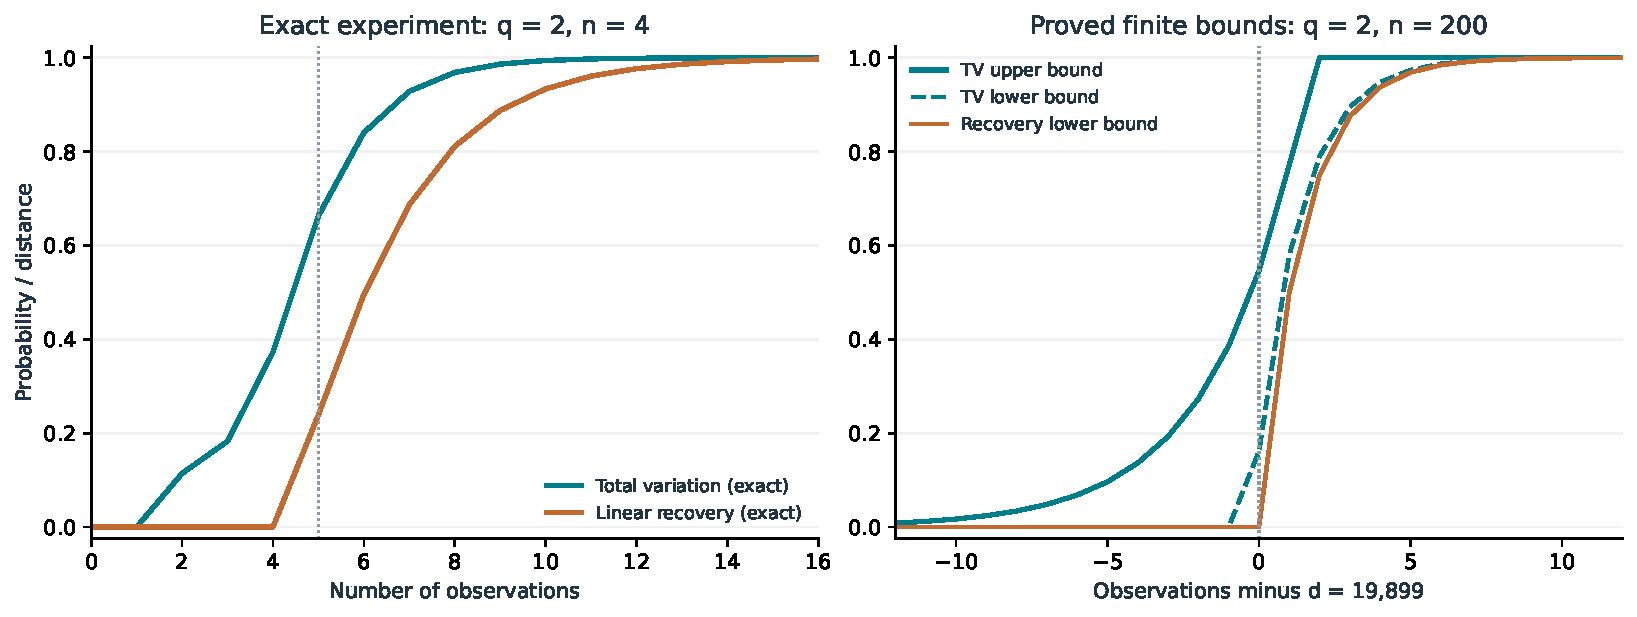
\includegraphics[width=\linewidth]{../figures/hidden_form_transition.pdf}
\caption{Left: exact finite probabilities for $q=2,n=4$, computed by integer state transitions. Right: explicit finite-dimensional inequalities for $q=2,n=200$, evaluated near $d=19899$. The right panel displays bounds, not simulations or limiting probability curves.}
\label{fig:transition}
\end{figure}

\subsection{What the checks establish}

The exact computations validate the combinatorial inputs, likelihood normalization, characteristic-two conventions, small-dimensional second moments, and the implemented recovery operation. They do not replace the asymptotic proof. That proof rests on the explicit bounds in \cref{hidden:prop:finite} and the separate treatment of proportional, near, and far competitors.

The right panel also has a directly certified finite interpretation. For $q=2,n=200$, there are $d=19899$ projective parameters. At $t=19889$, the finite inequalities certify total variation below $0.0171$ and optimal exact recovery probability below $0.001165$. At $t=19909$, they certify Gaussian recovery failure below $0.000977$, while its null-model false-positive probability is below $0.00082$. These rounded bounds are verified by exact rational comparisons in \texttt{code/make\_hidden\_figure.py}; it uses finite-product lower bounds, Bernoulli's inequality, and $e^x\le(1-x)^{-1}$ for $0\le x<1$. The curves in the figure are supplementary; all inequalities used for the theorem are proved symbolically.

\section{Scope and further questions}

The threshold theorem applies to a uniformly hidden nondegenerate form shared across conditionally independent isotropic-plane observations. Its recovery guarantee is uniform in the fixed hidden form. Its indistinguishability statement is a mixture statement with the specified uniform prior. The exact equivalence with matrix compressions includes full-row-rank conditioning. It therefore resolves a concrete case of the repository's unknown-source question, while the model with unconditioned blocks, arbitrary growing kernel dimensions, or noisy observations remains open.

The exact limit in \cref{hidden:thm:window} is a second-moment limit. It does not identify the limiting total variation or the full distribution of the compatible-form count $Z$ for $t=d+a$. Determining that law would give a more detailed transition profile. Another natural extension replaces two-planes by larger isotropic subspaces, which each impose several mutually dependent linear constraints.

The accompanying \texttt{FORMALIZATION.md} separates a possible Lean development into finite-field linear algebra, subspace counting, exact probability identities, and asymptotic estimates. No unproved formal statement is presented as a checked theorem.

\begin{thebibliography}{9}
\small\raggedright
\bibitem{proveit}
V. Reshetnikov, \emph{ProveIt: Generalized Riemann Hypothesis}, revision
\texttt{00cadb961bbe77c74e5d082c4948f8884d58a970}, 27 November 2026.
\url{https://github.com/VladimirReshetnikov/ProveIt/tree/00cadb961bbe77c74e5d082c4948f8884d58a970/Analysis/GeneralizedRiemannHypothesis}.
In particular \texttt{Article/sections/spn.tex}, labels \texttt{spn:thm:wide}, \texttt{spn:thm:wide-sample}, and \texttt{spn:q:symplectic}; and the three current packets \texttt{rectangular\_symplectic\_blocks}, \texttt{uniform\_symplectic\_blocks}, and \texttt{grh\_uniform\_extensions\_2026-11-27}.
\bibitem{cardinali}
I. Cardinali and L. Giuzzi, \emph{Minimum distance of symplectic Grassmann codes}, Linear Algebra and its Applications \textbf{488} (2016), 124--134.
\url{https://doi.org/10.1016/j.laa.2015.09.031}; \url{https://arxiv.org/abs/1503.05456}.
\bibitem{blok}
R. J. Blok, \emph{The generating rank of the symplectic line-Grassmannian}, Beitr\"age zur Algebra und Geometrie \textbf{44} (2003), 575--580.
\url{https://www.maths.tcd.ie/EMIS/journals/BAG/vol.44/no.2/26.html}.
\end{thebibliography}
\end{document}
